% Construction of the embedding matrix T of the embedded Trefftz DG method.
% Compile with: pdflatex Tmatrix.tex && pdftocairo -svg Tmatrix.pdf Tmatrix.svg
% (same workflow as Poly.tex)
\documentclass[tikz,border=4pt]{standalone}
\usepackage{amsmath,amssymb,bm}
\usetikzlibrary{arrows.meta,calc,decorations.pathreplacing}

% deck colors (css/style.css)
\definecolor{GOE}{RGB}{35,95,150}
\definecolor{navyblue}{RGB}{10,40,100}
\definecolor{alertred}{RGB}{179,32,32}
\definecolor{tgreen}{RGB}{22,135,111}

\newcommand{\A}{\mathcal{A}}
\newcommand{\Th}{\mathcal{T}_h}

\begin{document}
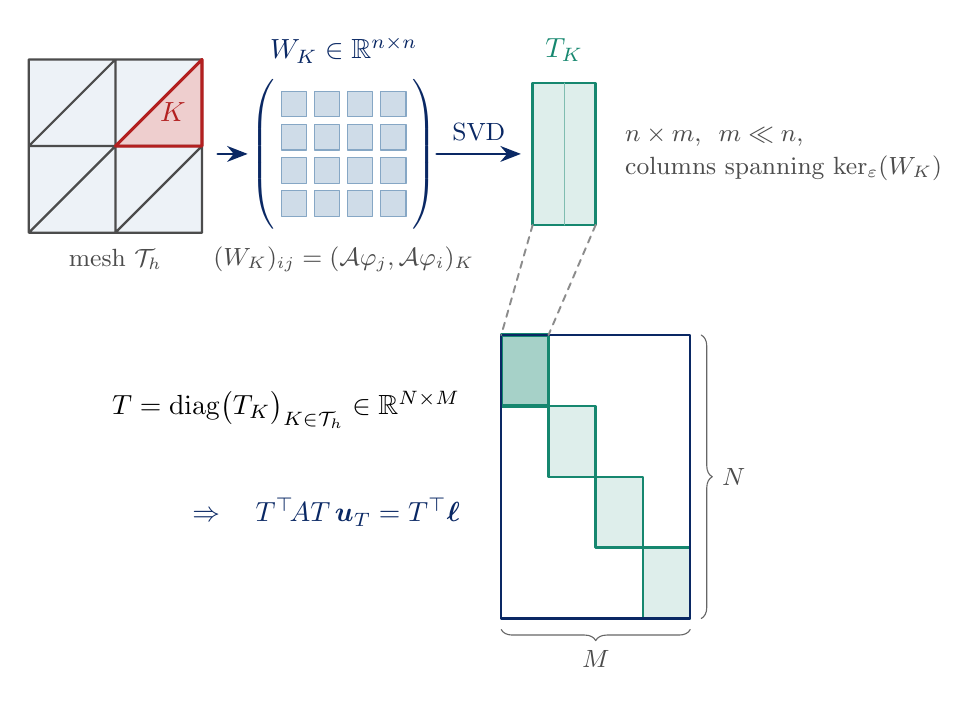
\begin{tikzpicture}[
    line join=round, line cap=round,
    font=\normalsize,
    mat/.style   = {draw=navyblue, line width=0.9pt, fill=GOE!10},
    ker/.style   = {draw=tgreen,   line width=0.9pt, fill=tgreen!14},
    kerhl/.style = {draw=tgreen,   line width=1.2pt, fill=tgreen!38},
    flow/.style  = {-{Stealth[length=2.6mm,width=2.0mm]}, line width=1pt, navyblue},
    zoom/.style  = {dashed, dash pattern=on 2.4pt off 2.2pt, line width=0.7pt, black!45},
    capt/.style  = {font=\small, text=black!70},
  ]

  %% ---------------------------------------------------------------- mesh
  \begin{scope}[shift={(0,4.9)}]
    \fill[GOE!8]  (0,0) rectangle (2.2,2.2);
    \fill[alertred!22] (1.1,1.1) -- (2.2,1.1) -- (2.2,2.2) -- cycle;
    \draw[line width=0.8pt, black!70]
        (0,0) rectangle (2.2,2.2)
        (1.1,0) -- (1.1,2.2)   (0,1.1) -- (2.2,1.1)
        (0,0) -- (1.1,1.1) -- (2.2,2.2)
        (1.1,0) -- (2.2,1.1)   (0,1.1) -- (1.1,2.2);
    \draw[alertred, line width=1.1pt] (1.1,1.1) -- (2.2,1.1) -- (2.2,2.2) -- cycle;
    \node[alertred] at (1.83,1.53) {$K$};
  \end{scope}
  \node[capt] at (1.1,4.56) {mesh $\Th$};

  %% ------------------------------------------------------- local matrix W_K
  %% a matrix, not a mesh: the entries are separate cells with air between them,
  %% inside round brackets sized by an invisible rule
  \foreach \i in {0,...,3} {
    \foreach \j in {0,...,3} {
      \fill[GOE!22, draw=GOE!55, line width=0.4pt]
        ({3.21+\i*0.42}, {5.11+\j*0.42}) rectangle ++(0.32,0.32);
    }
  }
  % inner sep=0: a tikz node's default padding is what pushes a delimiter away
  % from what it encloses, and here the brackets should sit on the cells
  \node[navyblue, anchor=east, inner sep=0pt] at (3.17,5.90)
       {$\left(\rule{0pt}{1.05cm}\right.$};
  \node[navyblue, anchor=west, inner sep=0pt] at (4.83,5.90)
       {$\left.\rule{0pt}{1.05cm}\right)$};
  \node[navyblue] at (4.0,7.22) {$W_K \in \mathbb{R}^{n\times n}$};
  \node[capt] at (4.0,4.56) {$(W_K)_{ij}=(\A\varphi_j,\A\varphi_i)_K$};

  %% ------------------------------------------------------------ local kernel
  \draw[ker] (6.4,5.0) rectangle (7.2,6.8);
  \draw[tgreen!55, line width=0.4pt] (6.8,5.0) -- (6.8,6.8);
  \node[tgreen] at (6.8,7.22) {$T_K$};
  \node[capt, anchor=west, align=left] at (7.45,5.9)
       {$n\times m$, \ $m \ll n$,\\[1pt] columns spanning $\ker_\varepsilon(W_K)$};

  %% ---------------------------------------------------------------- arrows
  \draw[flow] (2.4,5.9) -- (2.78,5.9);
  \draw[flow] (5.18,5.9) -- (6.25,5.9)
        node[midway, above=1pt, font=\small, text=navyblue] {SVD};

  %% ------------------------------------------------------------- global T
  \foreach \k in {0,1,2,3} {
    \pgfmathsetmacro{\bx}{6.0+0.6*\k}
    \pgfmathsetmacro{\by}{3.6-0.9*(\k+1)}
    \ifnum\k=0
      \draw[kerhl] (\bx,\by) rectangle ++(0.6,0.9);
    \else
      \draw[ker] (\bx,\by) rectangle ++(0.6,0.9);
    \fi
  }
  \draw[navyblue, line width=0.9pt] (6.0,0.0) rectangle (8.4,3.6);

  %% zoom from T_K down onto its block in T
  \draw[zoom] (6.4,5.0) -- (6.0,3.6);
  \draw[zoom] (7.2,5.0) -- (6.6,3.6);

  %% braces for N and M
  \draw[decorate, decoration={brace, amplitude=4pt}, black!60]
       (8.54,3.6) -- (8.54,0.0) node[midway, right=4pt, font=\small, text=black!70] {$N$};
  \draw[decorate, decoration={brace, amplitude=4pt, mirror}, black!60]
       (6.0,-0.14) -- (8.4,-0.14) node[midway, below=4pt, font=\small, text=black!70] {$M$};

  %% ------------------------------------------------------------- left labels
  \node[anchor=east] at (5.6,2.65)
       {$T=\operatorname{diag}\bigl(T_K\bigr)_{K\in\Th}\in\mathbb{R}^{N\times M}$};
  \node[anchor=east, text=navyblue] at (5.6,1.35)
       {$\Rightarrow\quad T^{\top}\!AT\,\bm{u}_T=T^{\top}\bm{\ell}$};

\end{tikzpicture}
\end{document}
